% $Id$
%


\usebackgroundtemplate{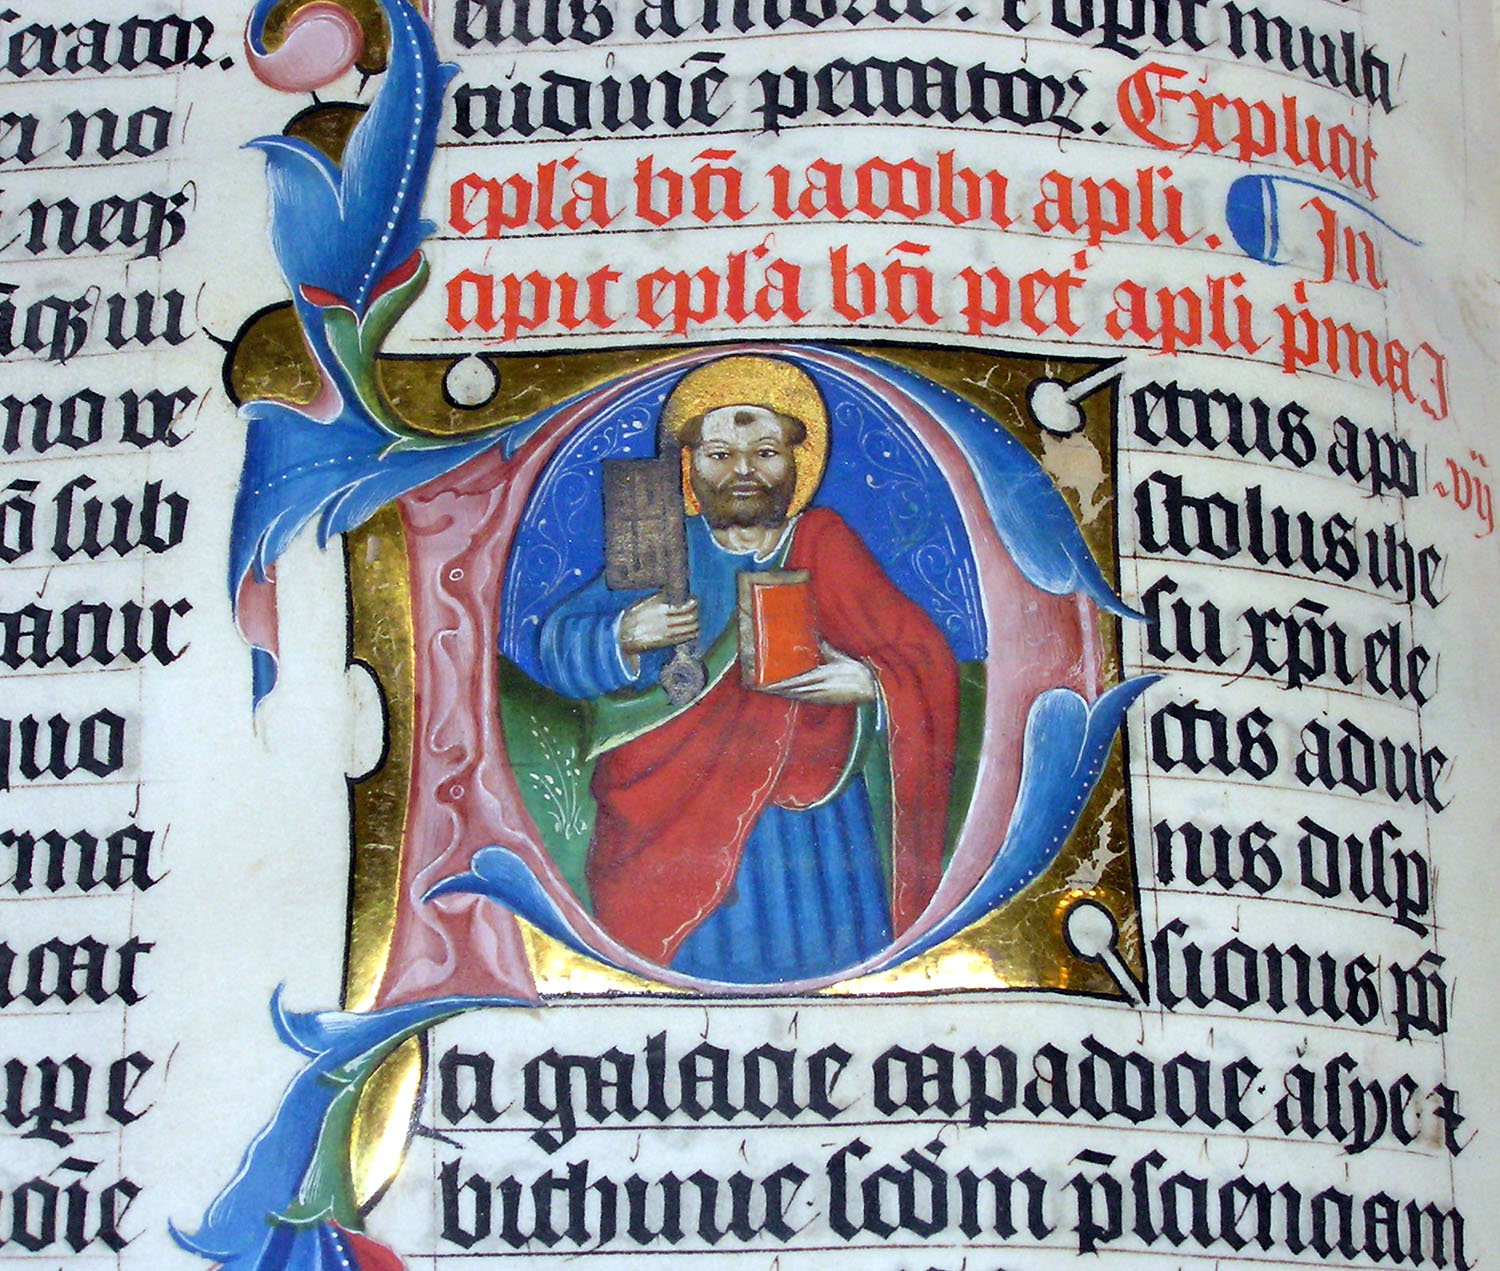
\includegraphics[width=13cm]{figs/biblia}}
{\bf
  \textcolor[rgb]{1,1,1}{
    \section{Documentos libres}
  }
}

\usebackgroundtemplate{}

%%---------------------------------------------------------------

\begin{frame}
\frametitle{Una excusa para promover una comunidad}

{\Large
\begin{itemize}
\item Un documento puede promover su propia ``comunidad de inter�s''
\item Si el documento es libre, la comunidad puede contribuir a su mejora
\item La comunidad puede no actuar de forma coordinada, ni en el mismo momento
\item El documento puede evolucionar de muchas formas (traducciones, actualizaciones, mezclas, mejoras)
\item En general, el documento conseguir� mucha m�s visbilidad.
\end{itemize}
}
\end{frame}

%%---------------------------------------------------------------

\begin{frame}
\frametitle{Requisitos b�sicos}

{\Large
Utilizar, modificar, redistribuir
\begin{flushright}
  ...aprovechar a otros, aprovecharse de otros
\end{flushright}

\vspace{.5cm}

\begin{itemize}
\item permisos legales (por el/los autores)
\item posibilidades t�cnicas
\end{itemize}
}
\end{frame}

%%---------------------------------------------------------------

\begin{frame}
\frametitle{Obras culturales libres}

{\Large

  Garant�a de las libertades b�sicas:
\begin{itemize}
\item Libertad de usar la obra
\item Libertad de estudiar la obra y aplicar lo aprendido
\item Libertad de hacer y redistribuir copias
\item Libertad de hacer cambios y mejoras
\end{itemize}


\includegraphics[width=3cm]{figs/free-cultural-works}

\begin{flushright}
  \url{http://freedomdefined.org/Definition/Es}
\end{flushright}
}

\end{frame}

%%---------------------------------------------------------------

\begin{frame}
\frametitle{Licencias libres}

{\Large

\begin{itemize}
\item Creative Commons Atribuci�n
\item Creative Commons Atribuci�n Compartir Igual
\item Obras en el dominio p�blico
\end{itemize}

\begin{flushright}
  \url{http://freedomdefined.org/Licenses} \\
  \url{http://creativecommons.org/freeworks} \\
\end{flushright}
}

\end{frame}

%%---------------------------------------------------------------

\begin{frame}
\frametitle{Consejos pr�cticos}

{\Large

\begin{itemize}
\item Utiliza una licencia libre y \\
  marca claramente la obra con ella
\item Reconoce las licencias (y la autor�a) \\
  de las obras que reutilices
\item Deja versiones modificables de la obra \\
  (editables si es texto, por ejemplo)
\end{itemize}

\begin{flushright}
  \url{http://freedomdefined.org/Licenses}
\end{flushright}
}

\end{frame}

%%---------------------------------------------------------------

\begin{frame}
\frametitle{Conseguir recursos libres (ejemplos:im�genes)}

{\Large

\begin{itemize}
\item Colecciones libres de Flickr \\
  (b�squeda avanzada, por licencia)
\item Wikimedia Commons
\item Google Images \\
  (herramientas de b�squeda, derechos de uso)
\end{itemize}

\begin{flushright}
  \url{http://flickr.com} \\
  \url{http://commons.wikimedia.org} \\
  \url{http://google.com} \\
\end{flushright}
}

\end{frame}



